% !TeX root = ../main.tex

\chapter{Experiments and Results}
\label{chap:results}

\newcolumntype{Y}{>{\centering\arraybackslash}p{0.18\linewidth}}

This chapter presents the five experiments listed in Section~\ref{sec:roadmap}. For each experiment, the configuration follows the description in Chapter~\ref{chap:methods}, and detailed numerical results are reported as tables and ROC curves to support the accompanying analysis.

\section{Experiment~1: Thumb-Tip Features vs.\ Bilateral Hand Joint Features}
\label{sec:exp1}

\subsection{Configuration}

In Experiment~1, two feature subsets are compared as input to three classical classifiers:
\begin{itemize}
    \item \textbf{Thumb-tip features.} Frequency, clarity, and amplitude features derived only from the thumb-tip trajectory (joint~4). The thumb tip is visually the most-displaced joint during pronation-supination and therefore a natural single-joint baseline.
    \item \textbf{Bilateral hand joint features.} The full 1{,}764-dimensional vector of features extracted from all 21 joints of both hands.
\end{itemize}

For each feature subset, Logistic Regression, Random Forest, and XGBoost are trained and evaluated under LOOCV on each cohort, and additionally under the 2020-to-2025 cross-cohort transfer protocol.

\subsection{Results}

Table~\ref{tab:thumb_model_comparison} reports the within-cohort LOOCV performance of the three classifiers on thumb-tip features. Table~\ref{tab:bilateral_model_comparison} reports the corresponding within-cohort results on bilateral hand-joint features. Figures~\ref{fig:thumb_roc_comparison} and~\ref{fig:bilateral_roc_comparison} show the corresponding ROC curves under both LOOCV and cross-cohort protocols. The explicit cross-cohort metrics (train on 2020, test on 2025) are summarized in Tables~\ref{tab:thumb_cross_dataset} and~\ref{tab:bilateral_cross_dataset}.

\begin{table}[H]
    \centering
    \caption{Within-cohort LOOCV performance of three classifiers on thumb-tip features}
    \label{tab:thumb_model_comparison}
    \small
    \setlength{\tabcolsep}{4pt}
    \begin{tabularx}{\linewidth}{>{\raggedright\arraybackslash}XYYY}
        \hline
        Model & \shortstack{AUROC\\(2020/2025)} & \shortstack{Accuracy\\(2020/2025)} & \shortstack{F1-score\\(2020/2025)} \\
        \hline
        Logistic Regression & 0.75 / 0.67 & 0.68 / 0.77 & 0.61 / 0.56 \\
        Random Forest       & 0.77 / 0.69 & 0.74 / 0.69 & 0.65 / 0.49 \\
        XGBoost             & 0.77 / 0.61 & 0.72 / 0.71 & 0.62 / 0.41 \\
        \hline
    \end{tabularx}
\end{table}

\begin{table}[H]
    \centering
    \caption{Within-cohort LOOCV performance of three classifiers on bilateral hand joint features}
    \label{tab:bilateral_model_comparison}
    \small
    \setlength{\tabcolsep}{4pt}
    \begin{tabularx}{\linewidth}{>{\raggedright\arraybackslash}XYYY}
        \hline
        Model & \shortstack{AUROC\\(2020/2025)} & \shortstack{Accuracy\\(2020/2025)} & \shortstack{F1-score\\(2020/2025)} \\
        \hline
        Logistic Regression & 0.81 / 0.67 & 0.79 / 0.80 & 0.67 / 0.50 \\
        Random Forest       & 0.82 / 0.71 & 0.73 / 0.71 & 0.66 / 0.51 \\
        XGBoost             & 0.77 / 0.62 & 0.74 / 0.73 & 0.61 / 0.47 \\
        \hline
    \end{tabularx}
\end{table}

\begin{table}[H]
    \centering
    \caption{Cross-cohort evaluation on thumb-tip features (train on 2020, test on 2025)}
    \label{tab:thumb_cross_dataset}
    \small
    \setlength{\tabcolsep}{4pt}
    \begin{tabularx}{\linewidth}{>{\raggedright\arraybackslash}XYYY}
        \hline
        Model & AUROC & Accuracy & F1-score \\
        \hline
        Logistic Regression & 0.63 & 0.52 & 0.46 \\
        Random Forest       & 0.71 & 0.51 & 0.46 \\
        XGBoost             & 0.71 & 0.51 & 0.44 \\
        \hline
    \end{tabularx}
\end{table}

\begin{table}[H]
    \centering
    \caption{Cross-cohort evaluation on bilateral hand joint features (train on 2020, test on 2025)}
    \label{tab:bilateral_cross_dataset}
    \small
    \setlength{\tabcolsep}{4pt}
    \begin{tabularx}{\linewidth}{>{\raggedright\arraybackslash}XYYY}
        \hline
        Model & AUROC & Accuracy & F1-score \\
        \hline
        Logistic Regression & 0.51 & 0.47 & 0.34 \\
        Random Forest       & 0.68 & 0.35 & 0.41 \\
        XGBoost             & 0.69 & 0.46 & 0.42 \\
        \hline
    \end{tabularx}
\end{table}

\begin{figure}[H]
    \centering
    \begin{subfigure}[b]{0.32\textwidth}
        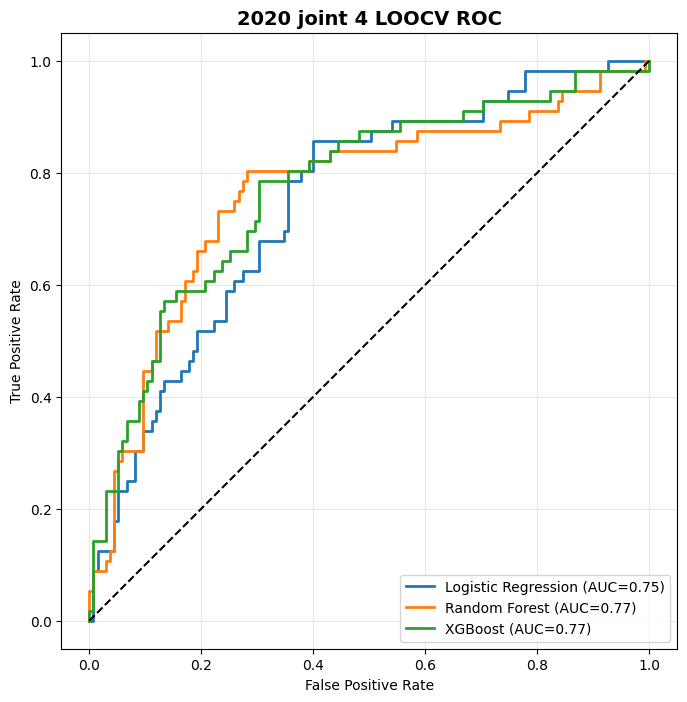
\includegraphics[width=\textwidth]{figures/2020_joint4.png}
        \caption{2020 (LOOCV) test}
        \label{fig:thumb_roc_2020}
    \end{subfigure}
    \hfill
    \begin{subfigure}[b]{0.32\textwidth}
        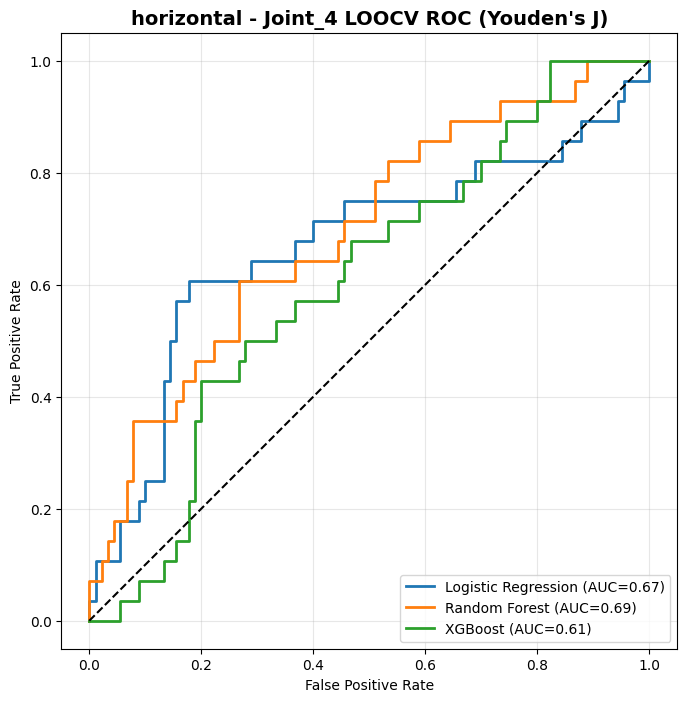
\includegraphics[width=\textwidth]{figures/2025_joint4.png}
        \caption{2025 (LOOCV)}
        \label{fig:thumb_roc_2025}
    \end{subfigure}
    \hfill
    \begin{subfigure}[b]{0.32\textwidth}
        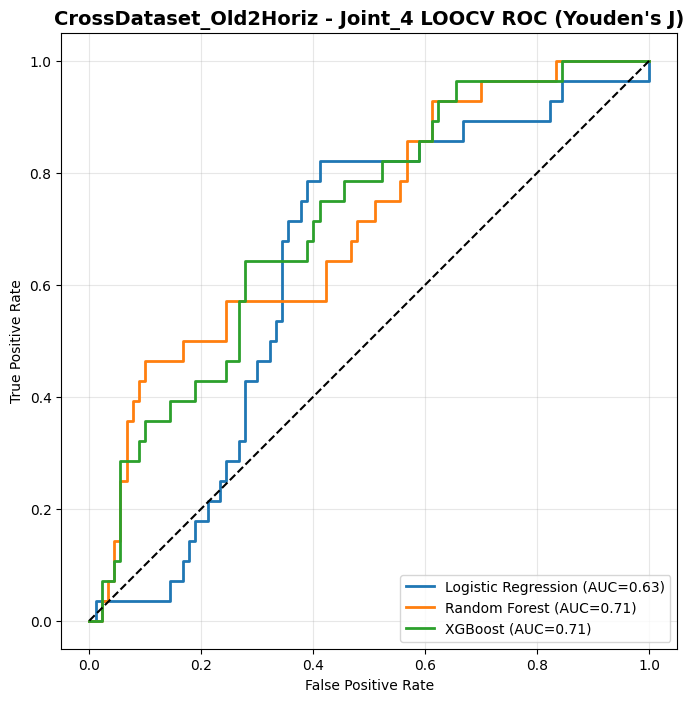
\includegraphics[width=\textwidth]{figures/cross_joint4.png}
        \caption{Cross-cohort}
        \label{fig:thumb_roc_cross}
    \end{subfigure}
    \caption{ROC curves on thumb-tip features under LOOCV and cross-cohort transfer.}
    \label{fig:thumb_roc_comparison}
\end{figure}

\begin{figure}[H]
    \centering
    \begin{subfigure}[t]{0.32\textwidth}
        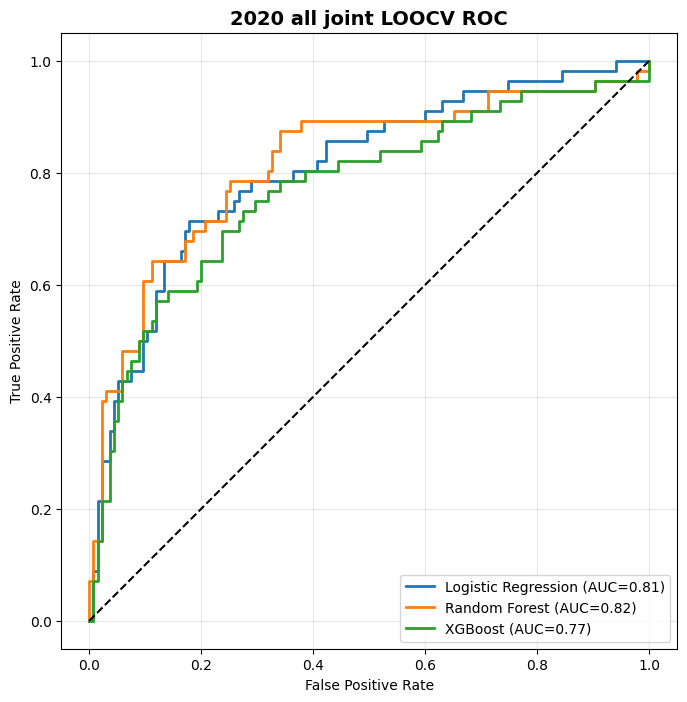
\includegraphics[width=\textwidth]{figures/2020_All_Joints.png}
        \caption{2020 (LOOCV)}
        \label{fig:bilateral_roc_2020}
    \end{subfigure}
    \hfill
    \begin{subfigure}[t]{0.32\textwidth}
        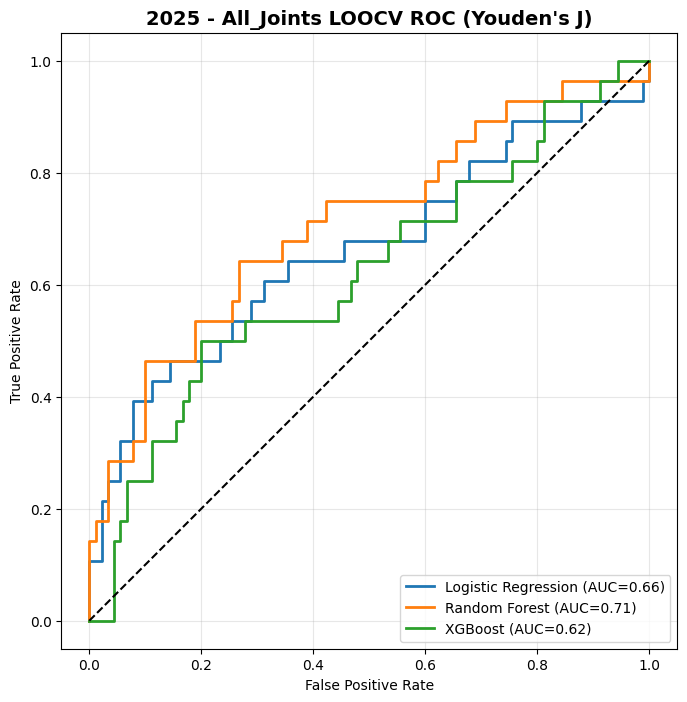
\includegraphics[width=\textwidth]{figures/2025_All_Joints.png}
        \caption{2025 (LOOCV)}
        \label{fig:bilateral_roc_2025}
    \end{subfigure}
    \hfill
    \begin{subfigure}[t]{0.32\textwidth}
        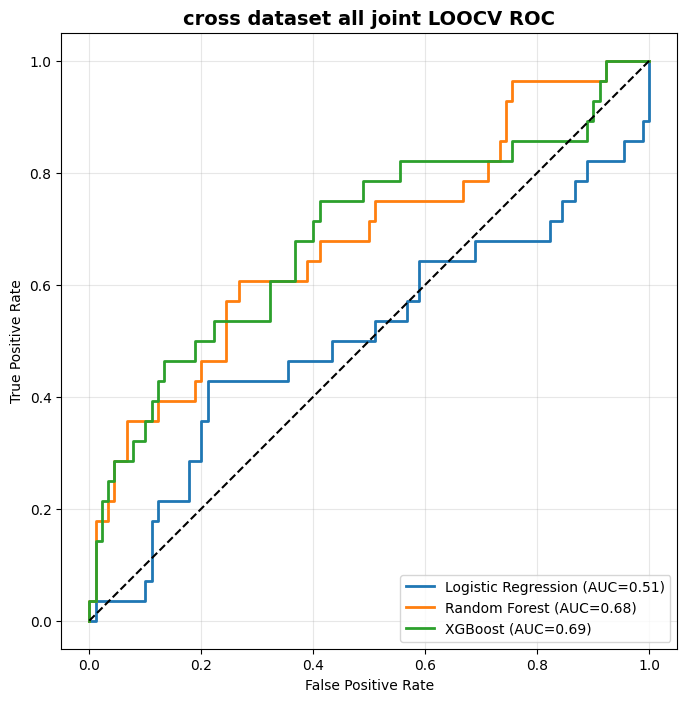
\includegraphics[width=\textwidth]{figures/cross_All_joints.png}
        \caption{Cross-cohort}
        \label{fig:bilateral_roc_cross}
    \end{subfigure}
    \caption{ROC curves on bilateral hand joint features under LOOCV and cross-cohort transfer.}
    \label{fig:bilateral_roc_comparison}
\end{figure}

\subsection{Observation}

Under LOOCV, performance on the 2020 and 2025 cohorts is broadly comparable across the two feature subsets and the three classifier families: thumb-tip features and bilateral features yield similar AUROC values, with no single classifier dominating in both cohorts simultaneously. In the cross-cohort transfer setting, however, XGBoost emerges as the most stable model in terms of AUROC, retaining $0.71$ on thumb-tip features and $0.69$ on bilateral features. This observation motivates the choice of XGBoost as the default downstream classifier for all subsequent experiments.

\section{Experiment~2: Feature Selection on Bilateral Hand Joint Features with XGBoost}
\label{sec:exp2}

\subsection{Configuration}

Experiment~2 builds on the bilateral feature subset of Experiment~1 by inserting an explicit feature-selection stage in front of the XGBoost classifier. The three feature-selection strategies introduced in Section~\ref{sec:fs} are compared: ANOVA F-value (\texttt{SelectKBest}), L1-regularized Logistic Regression, and XGBoost gain-based importance. The downstream classifier remains XGBoost. Feature selection is re-run inside every LOOCV training fold.

\subsection{Results}

Table~\ref{tab:fs_xgb_bilateral_comparison} reports the within-cohort LOOCV performance of the three feature-selection methods combined with XGBoost. Figure~\ref{fig:fs_bilateral_roc_comparison} shows the corresponding ROC curves, and Figure~\ref{fig:fs_bilateral_scatter_comparison} shows two-dimensional scatter plots of the most discriminative selected features. The cross-cohort transfer results are summarized in Table~\ref{tab:fs_bilateral_cross_dataset}.

\begin{table}[H]
    \centering
    \caption{Feature selection on bilateral features combined with XGBoost (LOOCV)}
    \label{tab:fs_xgb_bilateral_comparison}
    \small
    \setlength{\tabcolsep}{4pt}
    \begin{tabularx}{\linewidth}{>{\raggedright\arraybackslash}XYYY}
        \hline
        Method & \shortstack{AUROC\\(2020/2025)} & \shortstack{Accuracy\\(2020/2025)} & \shortstack{F1-score\\(2020/2025)} \\
        \hline
        ANOVA + XGBoost              & 0.74 / 0.62 & 0.76 / 0.48 & 0.64 / 0.45 \\
        L1-Logistic + XGBoost        & 0.74 / 0.57 & 0.80 / 0.62 & 0.61 / 0.43 \\
        XGB Importance + XGBoost     & 0.74 / 0.69 & 0.78 / 0.73 & 0.60 / 0.54 \\
        \hline
    \end{tabularx}
\end{table}

\begin{table}[H]
    \centering
    \caption{Cross-cohort evaluation of feature selection on bilateral features with XGBoost (train on 2020, test on 2025)}
    \label{tab:fs_bilateral_cross_dataset}
    \small
    \setlength{\tabcolsep}{4pt}
    \begin{tabularx}{\linewidth}{>{\raggedright\arraybackslash}XYYY}
        \hline
        Method & AUROC & Accuracy & F1-score \\
        \hline
        ANOVA + XGBoost              & 0.68 & 0.52 & 0.42 \\
        L1-Logistic + XGBoost        & 0.68 & 0.66 & 0.46 \\
        XGB Importance + XGBoost     & 0.65 & 0.56 & 0.41 \\
        \hline
    \end{tabularx}
\end{table}

\begin{figure}[H]
    \centering
    \begin{subfigure}[t]{0.32\textwidth}
        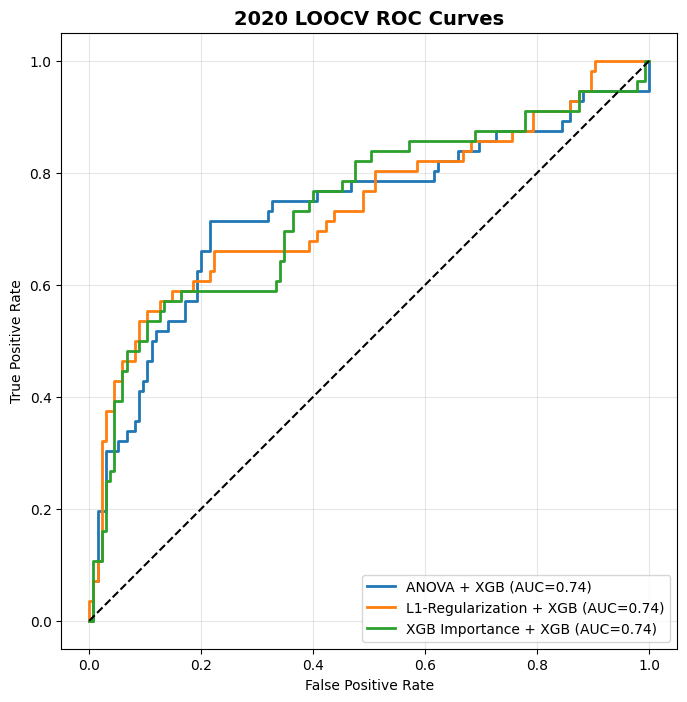
\includegraphics[width=\textwidth]{figures/2020_fs_bilateral.png}
        \caption{2020 (LOOCV)}
        \label{fig:fs_bilateral_roc_2020}
    \end{subfigure}
    \hfill
    \begin{subfigure}[t]{0.32\textwidth}
        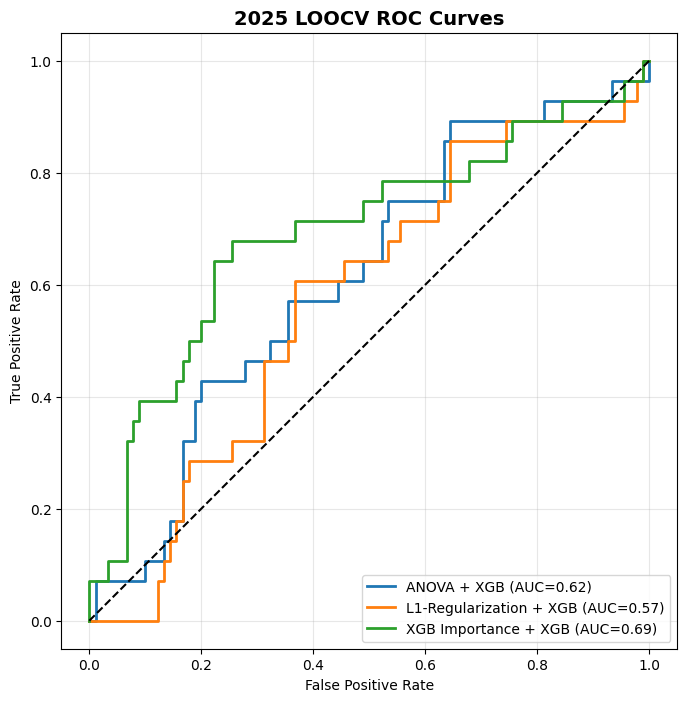
\includegraphics[width=\textwidth]{figures/2025_fs_bilateral.png}
        \caption{2025 (LOOCV)}
        \label{fig:fs_bilateral_roc_2025}
    \end{subfigure}
    \hfill
    \begin{subfigure}[t]{0.32\textwidth}
        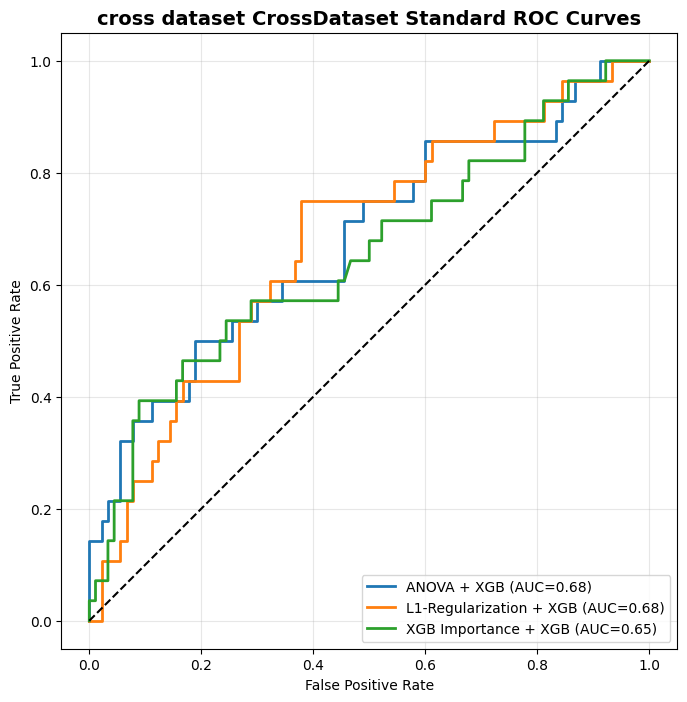
\includegraphics[width=\textwidth]{figures/cross_fs_bilateral.png}
        \caption{Cross-cohort}
        \label{fig:fs_bilateral_roc_cross}
    \end{subfigure}
    \caption{ROC curves of feature selection on bilateral features combined with XGBoost.}
    \label{fig:fs_bilateral_roc_comparison}
\end{figure}

\begin{figure}[H]
    \centering
    \begin{subfigure}[t]{0.32\textwidth}
        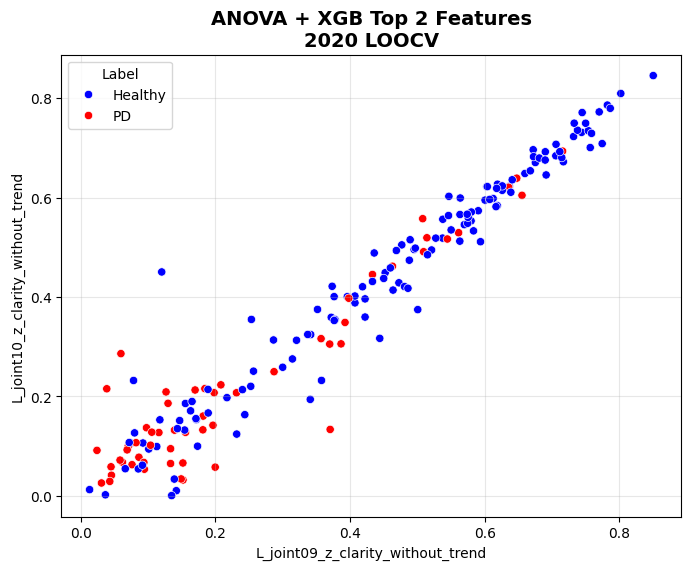
\includegraphics[width=\textwidth]{figures/2020_anova_fs_scatter.png}
        \caption{ANOVA, 2020}
    \end{subfigure}
    \hfill
    \begin{subfigure}[t]{0.32\textwidth}
        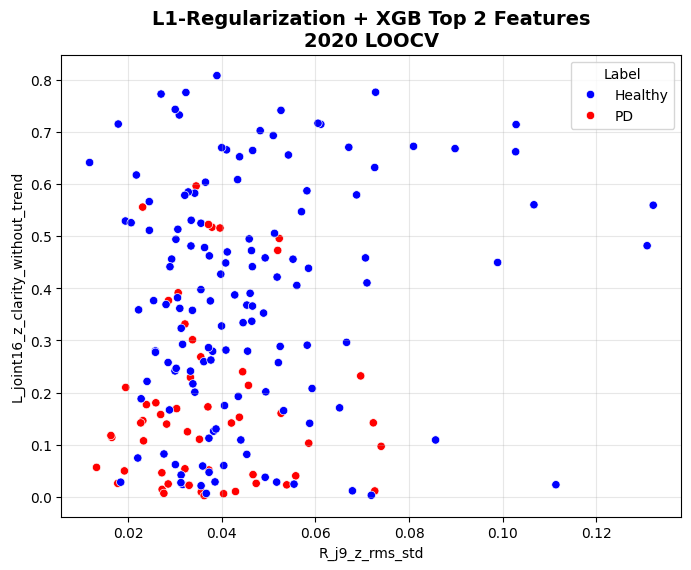
\includegraphics[width=\textwidth]{figures/2020_l1_fs_scatter.png}
        \caption{L1-Logistic, 2020}
    \end{subfigure}
    \hfill
    \begin{subfigure}[t]{0.32\textwidth}
        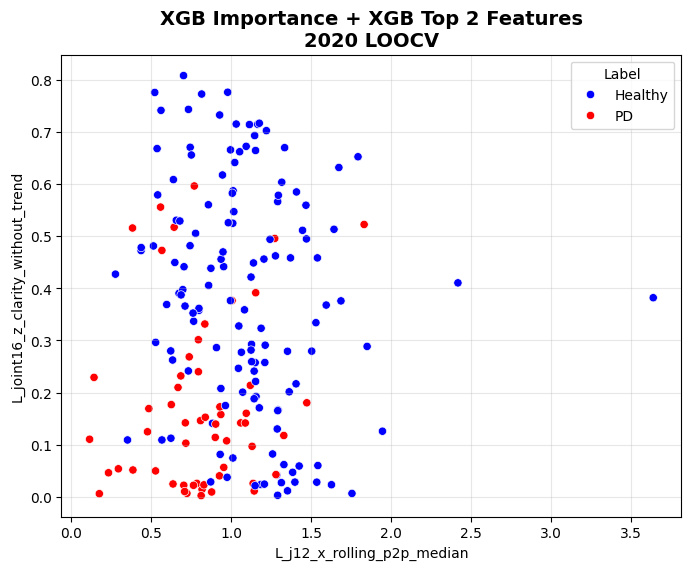
\includegraphics[width=\textwidth]{figures/2020_xgbimp_fs_scatter.png}
        \caption{XGB Importance, 2020}
    \end{subfigure}

    \vspace{0.2em}

    \begin{subfigure}[t]{0.32\textwidth}
        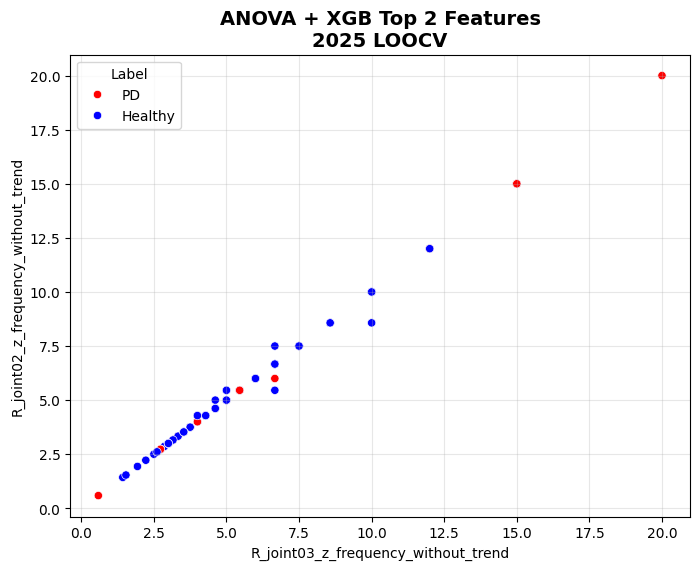
\includegraphics[width=\textwidth]{figures/2025_anova_fs_scatter.png}
        \caption{ANOVA, 2025}
    \end{subfigure}
    \hfill
    \begin{subfigure}[t]{0.32\textwidth}
        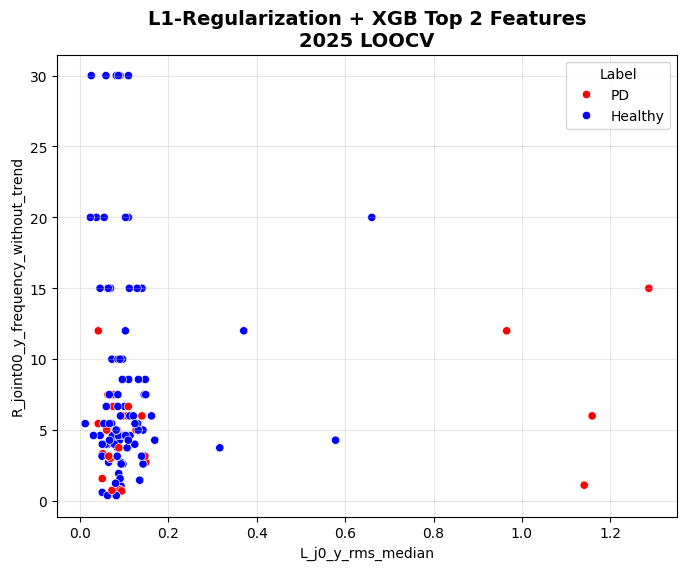
\includegraphics[width=\textwidth]{figures/2025_l1_fs_scatter.png}
        \caption{L1-Logistic, 2025}
    \end{subfigure}
    \hfill
    \begin{subfigure}[t]{0.32\textwidth}
        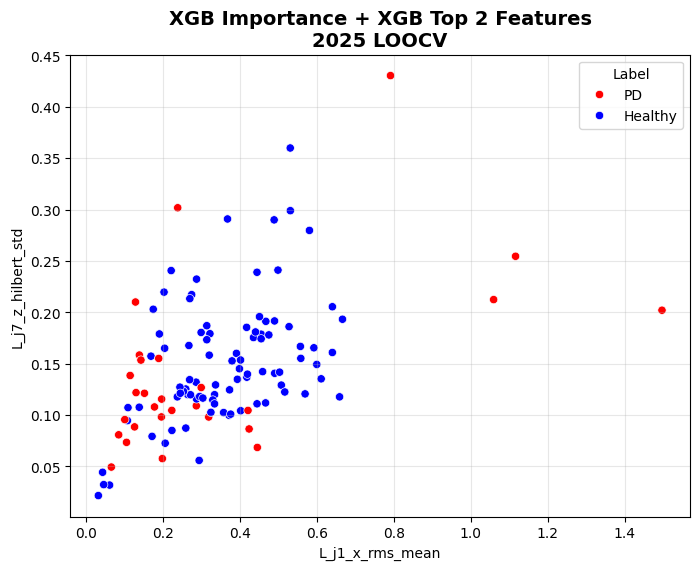
\includegraphics[width=\textwidth]{figures/2025_xgbimp_fs_scatter.png}
        \caption{XGB Importance, 2025}
    \end{subfigure}
    \caption{Scatter plots of the most discriminative selected features for the three feature-selection methods on bilateral features (PD vs healthy).}
    \label{fig:fs_bilateral_scatter_comparison}
\end{figure}

\subsection{Top-10 Hand-Side Distribution}

To investigate which hand contributes most of the discriminative signal, the top-10 selected features are first aggregated across LOOCV folds for each feature-selection method. The counts in Table~\ref{tab:fs_topk_hand_distribution} then sum these top-10 lists across the three methods, so each cohort contributes 30 selected-feature slots rather than a single set of 10 features.

\begin{table}[H]
    \centering
    \caption{Aggregated distribution of top-10 selected features across the three feature-selection methods}
    \label{tab:fs_topk_hand_distribution}
    \small
    \setlength{\tabcolsep}{8pt}
    \begin{tabularx}{\linewidth}{>{\raggedright\arraybackslash}X c c}
        \hline
        Cohort & Right-hand count & Left-hand count \\
        \hline
        2020 & 5  & 25 \\
        2025 & 11 & 19 \\
        \hline
    \end{tabularx}
\end{table}

\subsection{Observation}

All three feature-selection methods reach the same AUROC of $0.74$ on the 2020 cohort. On the 2025 cohort, XGBoost Importance yields the strongest within-cohort generalization, with the highest AUROC ($0.69$), accuracy ($0.73$), and F1-score ($0.54$). In the cross-cohort transfer setting, ANOVA and L1-Logistic feature selection retain the highest AUROC of $0.68$, but the threshold-dependent accuracy and F1-score remain modest, indicating that transfer across cohorts is still difficult.

The hand-side distribution in Table~\ref{tab:fs_topk_hand_distribution} reveals a consistent left-versus-right asymmetry across the 30 selected-feature slots: the left hand contributes $25{:}5$ on the 2020 cohort and $19{:}11$ on the 2025 cohort. This observation directly motivates Experiment~3.

\section{Experiment~3: Left-Hand-Only vs.\ Right-Hand-Only Feature Selection with XGBoost}
\label{sec:exp3}

\subsection{Configuration}

Experiment~3 repeats the feature-selection-plus-XGBoost pipeline of Experiment~2 on three feature subsets: the left-hand-only subset, the right-hand-only subset, and the bilateral subset (the latter is included for reference). All other settings, including LOOCV protocol and cross-cohort transfer, are identical to Experiment~2.

\subsection{Results}

Tables~\ref{tab:fs_xgb_right_hand_comparison} and~\ref{tab:fs_xgb_left_hand_comparison} report the within-cohort LOOCV performance for the right and left hand respectively, and Figure~\ref{fig:fs_hand_roc_comparison} shows the corresponding ROC curves. The cross-cohort transfer results are summarized in Table~\ref{tab:fs_lr_hand_cross_dataset}.

\begin{table}[H]
    \centering
    \caption{Right-hand-only feature selection combined with XGBoost (LOOCV)}
    \label{tab:fs_xgb_right_hand_comparison}
    \small
    \setlength{\tabcolsep}{4pt}
    \begin{tabularx}{\linewidth}{>{\raggedright\arraybackslash}XYYY}
        \hline
        Method & \shortstack{AUROC\\(2020/2025)} & \shortstack{Accuracy\\(2020/2025)} & \shortstack{F1-score\\(2020/2025)} \\
        \hline
        ANOVA + XGBoost              & 0.57 / 0.67 & 0.66 / 0.69 & 0.40 / 0.45 \\
        L1-Logistic + XGBoost        & 0.70 / 0.77 & 0.62 / 0.64 & 0.55 / 0.53 \\
        XGB Importance + XGBoost     & 0.68 / 0.56 & 0.66 / 0.70 & 0.53 / 0.36 \\
        \hline
    \end{tabularx}
\end{table}

\begin{table}[H]
    \centering
    \caption{Left-hand-only feature selection combined with XGBoost (LOOCV)}
    \label{tab:fs_xgb_left_hand_comparison}
    \small
    \setlength{\tabcolsep}{4pt}
    \begin{tabularx}{\linewidth}{>{\raggedright\arraybackslash}XYYY}
        \hline
        Method & \shortstack{AUROC\\(2020/2025)} & \shortstack{Accuracy\\(2020/2025)} & \shortstack{F1-score\\(2020/2025)} \\
        \hline
        ANOVA + XGBoost              & 0.74 / 0.53 & 0.76 / 0.63 & 0.64 / 0.39 \\
        L1-Logistic + XGBoost        & 0.78 / 0.63 & 0.79 / 0.70 & 0.66 / 0.44 \\
        XGB Importance + XGBoost     & 0.76 / 0.75 & 0.82 / 0.81 & 0.65 / 0.63 \\
        \hline
    \end{tabularx}
\end{table}

\begin{table}[H]
    \centering
    \caption{Cross-cohort evaluation of right- and left-hand-only feature selection with XGBoost (train on 2020, test on 2025)}
    \label{tab:fs_lr_hand_cross_dataset}
    \small
    \setlength{\tabcolsep}{4pt}
    \begin{tabularx}{\linewidth}{>{\raggedleft\arraybackslash}p{0.15\linewidth}XYYY}
        \hline
        & Method & AUROC & Accuracy & F1-score \\
        \hline
        \multirow{3}{*}{Right hand} & ANOVA + XGBoost           & 0.68 & 0.66 & 0.41 \\
                                    & L1-Logistic + XGBoost     & 0.62 & 0.42 & 0.38 \\
                                    & XGB Importance + XGBoost  & 0.65 & 0.52 & 0.39 \\
        \hline
        \multirow{3}{*}{Left hand}  & ANOVA + XGBoost           & 0.68 & 0.52 & 0.42 \\
                                    & L1-Logistic + XGBoost     & 0.64 & 0.63 & 0.41 \\
                                    & XGB Importance + XGBoost  & 0.66 & 0.65 & 0.47 \\
        \hline
    \end{tabularx}
\end{table}

\begin{figure}[H]
    \centering
    \begin{subfigure}[t]{0.32\textwidth}
        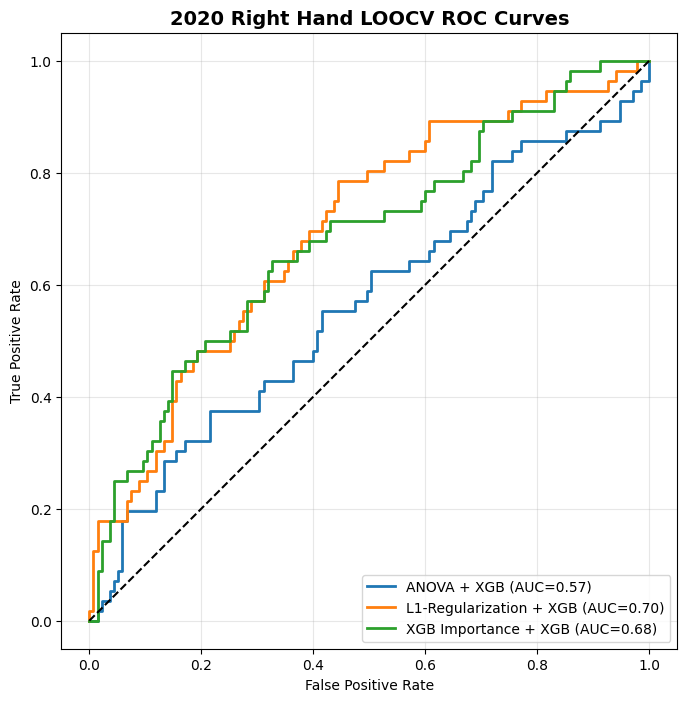
\includegraphics[width=\textwidth]{figures/2020_right_hand_fs.png}
        \caption{Right hand, 2020}
    \end{subfigure}
    \hfill
    \begin{subfigure}[t]{0.32\textwidth}
        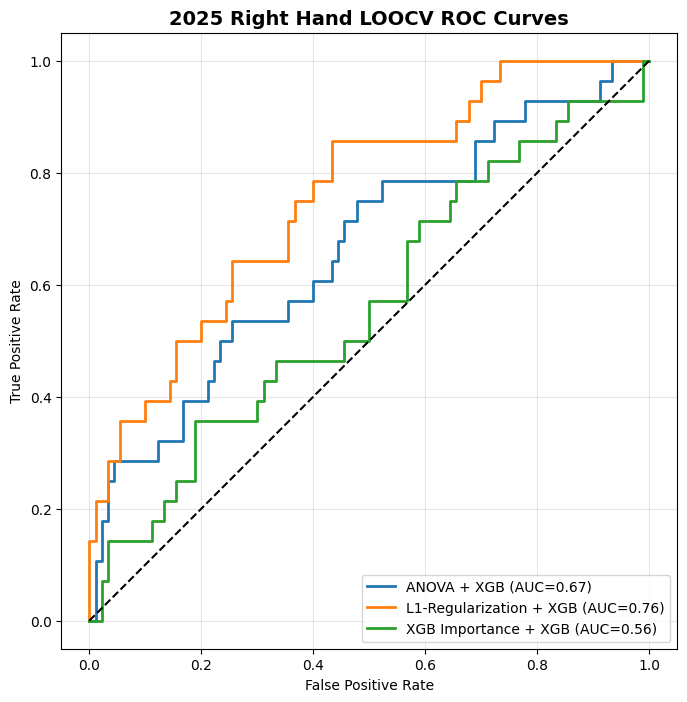
\includegraphics[width=\textwidth]{figures/2025_right_hand_fs.png}
        \caption{Right hand, 2025}
    \end{subfigure}
    \hfill
    \begin{subfigure}[t]{0.32\textwidth}
        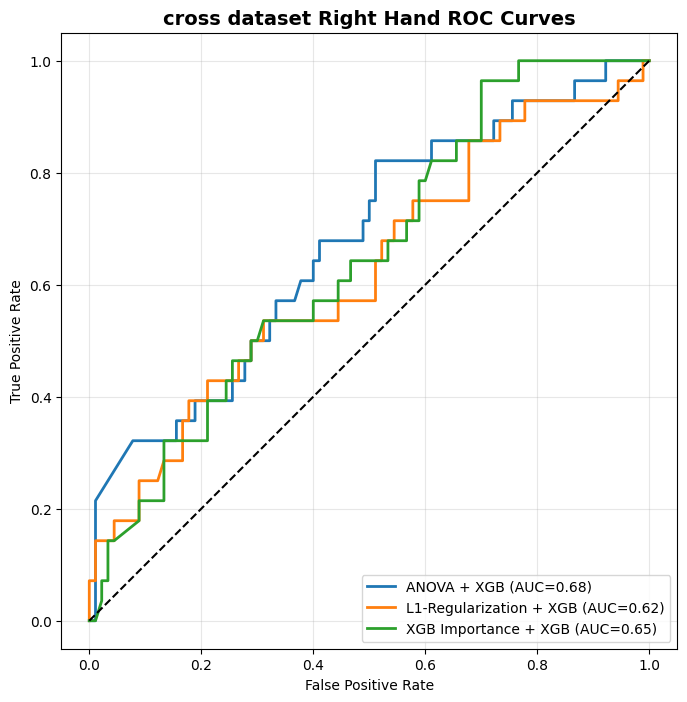
\includegraphics[width=\textwidth]{figures/cross_right_hand_fs.png}
        \caption{Right hand, cross-cohort}
    \end{subfigure}

    \vspace{0.2em}

    \begin{subfigure}[t]{0.32\textwidth}
        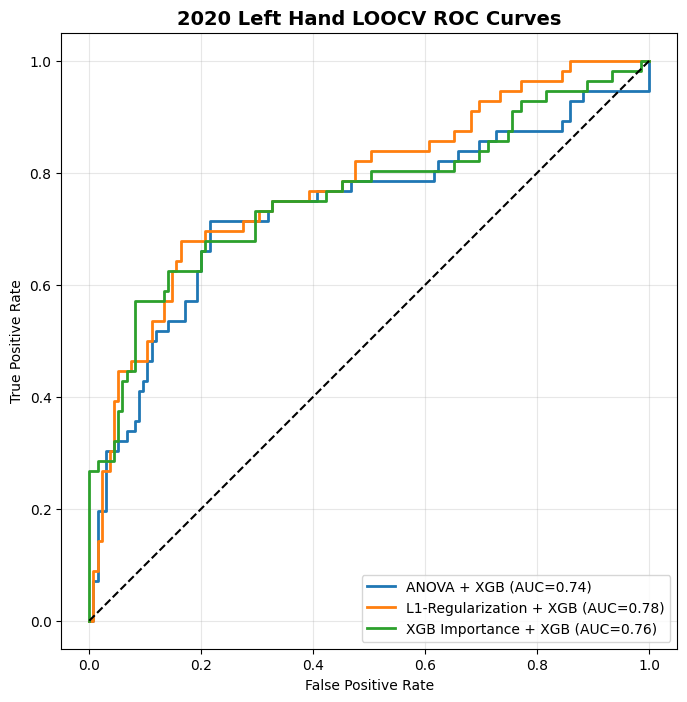
\includegraphics[width=\textwidth]{figures/2020_left_hand_fs.png}
        \caption{Left hand, 2020}
    \end{subfigure}
    \hfill
    \begin{subfigure}[t]{0.32\textwidth}
        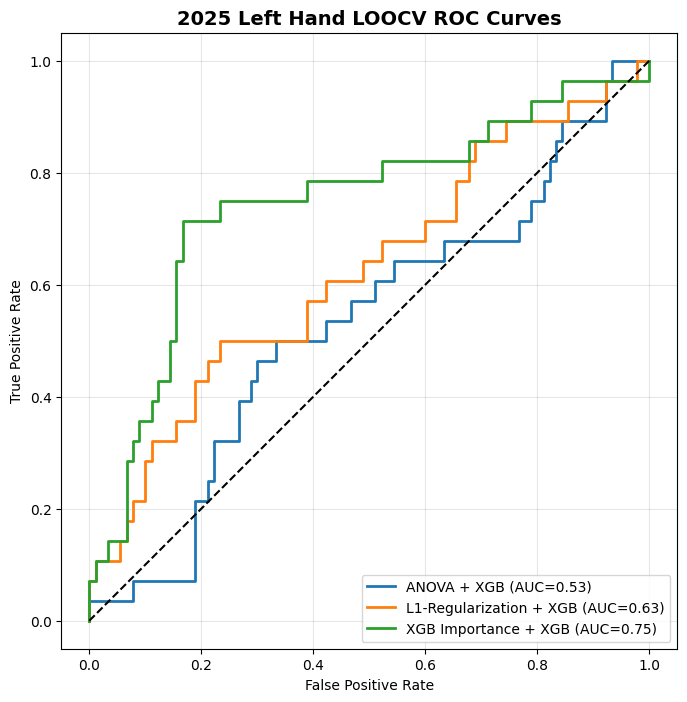
\includegraphics[width=\textwidth]{figures/2025_left_hand_fs.png}
        \caption{Left hand, 2025}
    \end{subfigure}
    \hfill
    \begin{subfigure}[t]{0.32\textwidth}
        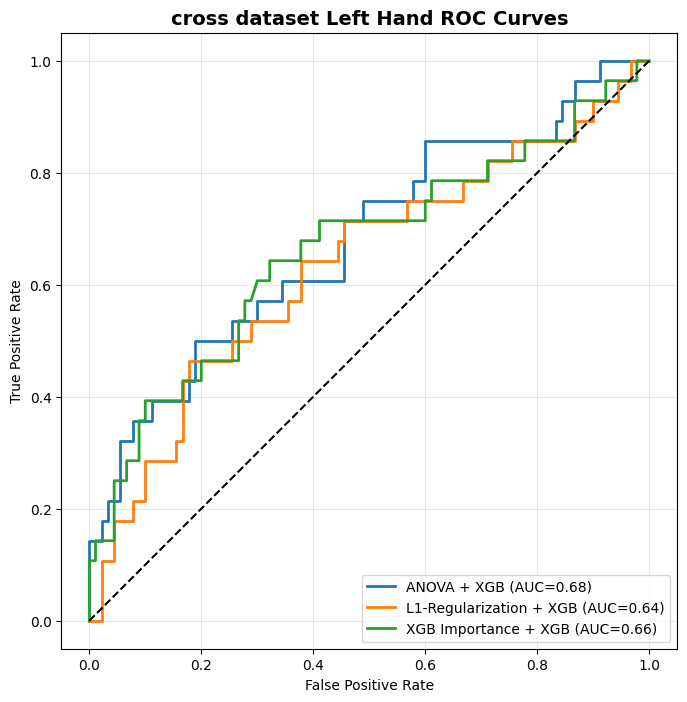
\includegraphics[width=\textwidth]{figures/cross_left_hand_fs.png}
        \caption{Left hand, cross-cohort}
    \end{subfigure}
    \caption{ROC curves of feature selection combined with XGBoost on right-hand-only and left-hand-only features.}
    \label{fig:fs_hand_roc_comparison}
\end{figure}

\subsection{Observation}

The left-hand XGB Importance + XGBoost configuration is the strongest single-hand baseline, reaching AUROCs of $0.76$ and $0.75$ on the 2020 and 2025 cohorts respectively, with accuracies of $0.82$ and $0.81$. The advantage is most consistent for the XGB-importance selector: it outperforms the corresponding right-hand configuration in both cohorts and also yields the highest cross-cohort F1-score among single-hand models. This pattern, together with the left-heavy top-feature distribution observed in Experiment~2, is consistent with a scenario in which the dominant hand retains more motor reserve and therefore shows less feature separation, while the non-dominant hand exhibits earlier and more detectable kinematic decline. However, this interpretation should be treated with caution. Because individual handedness was not recorded, it cannot be established that the left hand was non-dominant for the majority of subjects in either cohort. The observed asymmetry may alternatively reflect population-level differences in how PD pathology progresses across the two sides, recording-specific confounds, or the particular joints and features selected by the XGB importance method. The finding is therefore reported as an empirical left-versus-right asymmetry in feature discriminability rather than as confirmatory evidence for the motor-reserve hypothesis.

\section{Experiment~4: Bilateral Features Plus Graph-Aggregated Joint-Correlation Features}
\label{sec:exp4}

\subsection{Configuration}

Experiment~4 evaluates whether the 203-dimensional graph-aggregated joint-correlation descriptor (Section~\ref{sec:joint_corr_corr}) adds discriminative value on top of the bilateral kinematic features. The bilateral feature vector is extended from 1,764 to 1,967 dimensions by appending the graph descriptor, which encodes inter-joint feature-profile similarity via a Ledoit-Wolf shrinkage correlation matrix, one step of GCN-style aggregation, node-level pooling statistics, bilateral asymmetry, and block-level intra/inter-hand coupling statistics. The three feature-selection strategies are then applied to reduce this extended space, and XGBoost is used as the downstream classifier. Two baselines are kept for comparison: the strongest single-side model from Experiment~3 (left-hand XGB Importance) and the strongest bilateral model from Experiment~2 (bilateral XGB Importance).

\subsection{Results}

Table~\ref{tab:correlation_within_cohort} reports the within-cohort LOOCV performance and Table~\ref{tab:correlation_cross_dataset} reports the cross-cohort transfer results.

\begin{table}[H]
    \centering
    \caption{Within-cohort LOOCV performance with graph-aggregated joint-correlation features added to the bilateral feature set}
    \label{tab:correlation_within_cohort}
    \small
    \setlength{\tabcolsep}{4pt}
    \begin{tabularx}{\linewidth}{>{\raggedright\arraybackslash}XYYY}
        \hline
        Method & \shortstack{AUROC\\(2020/2025)} & \shortstack{Accuracy\\(2020/2025)} & \shortstack{F1-score\\(2020/2025)} \\
        \hline
        Left-hand XGB Importance (baseline)         & 0.76 / 0.75 & 0.82 / 0.81 & 0.65 / 0.63 \\
        Bilateral XGB Importance (baseline)         & 0.74 / 0.69 & 0.78 / 0.73 & 0.60 / 0.54 \\
        Graph-Corr + ANOVA + XGBoost               & 0.74 / 0.61 & 0.77 / 0.63 & 0.63 / 0.44 \\
        Graph-Corr + L1-Logistic + XGBoost         & 0.72 / 0.56 & 0.79 / 0.60 & 0.62 / 0.42 \\
        Graph-Corr + XGB Importance + XGBoost      & 0.73 / 0.66 & 0.78 / 0.61 & 0.60 / 0.48 \\
        \hline
    \end{tabularx}
\end{table}

\begin{table}[H]
    \centering
    \caption{Cross-cohort evaluation with graph-aggregated joint-correlation features (train on 2020, test on 2025)}
    \label{tab:correlation_cross_dataset}
    \small
    \setlength{\tabcolsep}{4pt}
    \begin{tabularx}{\linewidth}{>{\raggedright\arraybackslash}XYYY}
        \hline
        Method & AUROC & Accuracy & F1-score \\
        \hline
        Left-hand XGB Importance (baseline)         & 0.66 & 0.65 & 0.47 \\
        Bilateral XGB Importance (baseline)         & 0.65 & 0.56 & 0.41 \\
        Graph-Corr + ANOVA + XGBoost               & 0.68 & 0.56 & 0.45 \\
        Graph-Corr + L1-Logistic + XGBoost         & 0.65 & 0.62 & 0.44 \\
        Graph-Corr + XGB Importance + XGBoost      & 0.67 & 0.58 & 0.45 \\
        \hline
    \end{tabularx}
\end{table}

\subsection{Observation}

Adding the 203-dimensional graph-aggregated joint-correlation descriptor does \emph{not} produce a consistent improvement over the strongest baselines. Within cohort, the best augmented configuration only matches the bilateral baseline (AUROC $0.74$) on the 2020 cohort and reaches AUROC $0.66$ on the 2025 cohort, both below the left-hand-only baseline (AUROC $0.75$). In the cross-cohort transfer setting, the ANOVA- and XGB-based augmented configurations yield AUROC of $0.68$ and $0.67$ respectively, marginally above the two baselines ($0.65$--$0.66$), but the L1-regularised configuration ($0.65$) does not improve over the bilateral baseline. Accuracy and F1-score show no consistent gain. We interpret this as evidence that, once autocorrelation and amplitude descriptors are in place, the additional graph-structured inter-joint correlation carries limited incremental discriminative information.

\section{Experiment~5: Adaptive Graph Convolutional Network}
\label{sec:exp5}

\subsection{Configuration}

Experiment~5 evaluates the feature-based AGCN-style model described in Section~\ref{sec:joint_corr_agcn}. The model uses the same 1,764-dimensional bilateral kinematic feature vector as the preceding feature-based experiments, but reorganises it as a 42-node joint graph rather than treating it as a flat tabular vector. The adaptive graph is derived from the layer-wise node-feature transformation through a Mahalanobis distance and Gaussian kernel, allowing the model to learn sample-dependent joint relations from the input representation. After graph propagation, the per-node embeddings are average-pooled into a graph-level representation and passed to a linear classification head. Henceforth this configuration is referred to simply as \emph{AGCN}.

The AGCN result is reported alongside the strongest baselines from Experiments~2--4: the bilateral XGB Importance baseline (Exp.~2), the left-hand XGB Importance baseline (Exp.~3), and the three correlation-augmented configurations (Exp.~4). All baselines use XGBoost as the downstream classifier.

\subsection{Results}

Table~\ref{tab:gcn_methods_2020} reports the 2020 within-cohort method comparison; Table~\ref{tab:gcn_methods_2025} reports the 2025 within-cohort method comparison; and Table~\ref{tab:gcn_cross_dataset} reports the 2020-to-2025 cross-cohort transfer comparison.

\begin{table}[H]
    \centering
    \caption{Method comparison on the 2020 cohort under LOOCV (AGCN vs.\ baselines from Exp.~2--4)}
    \label{tab:gcn_methods_2020}
    \small
    \setlength{\tabcolsep}{4pt}
    \begin{tabularx}{\linewidth}{>{\raggedright\arraybackslash}XYYY}
        \hline
        Method & AUROC & Accuracy & F1-score \\
        \hline
        Left-hand XGB Importance             & 0.76 & 0.82 & 0.65 \\
        XGB Importance                       & 0.74 & 0.78 & 0.60 \\
        Graph-Corr + ANOVA                   &0.74 & 0.77 & 0.63 \\
        Graph-Corr + Logistic L1             &0.72 & 0.79 & 0.62 \\
        Graph-Corr + XGB Importance          &0.73 & 0.78 & 0.60 \\
        AGCN                                 & 0.98 & 0.93 & 0.89 \\
        \hline
    \end{tabularx}
\end{table}

\begin{table}[H]
    \centering
    \caption{Method comparison on the 2025 cohort under LOOCV (AGCN vs.\ baselines from Exp.~2--4)}
    \label{tab:gcn_methods_2025}
    \small
    \setlength{\tabcolsep}{4pt}
    \begin{tabularx}{\linewidth}{>{\raggedright\arraybackslash}XYYY}
        \hline
        Method & AUROC & Accuracy & F1-score \\
        \hline
        Left-hand XGB Importance             & 0.75 & 0.81 & 0.63 \\
        XGB Importance                       & 0.69 & 0.73 & 0.54 \\
        Graph-Corr + ANOVA                   &0.61 & 0.63 & 0.44 \\
        Graph-Corr + Logistic L1             &0.56 & 0.60 & 0.42 \\
        Graph-Corr + XGB Importance          &0.66 & 0.61 & 0.48 \\
        AGCN                                 & 0.98 & 0.92 & 0.85 \\
        \hline
    \end{tabularx}
\end{table}

\begin{table}[H]
    \centering
    \caption{Method comparison under cross-cohort evaluation (train on 2020, test on 2025)}
    \label{tab:gcn_cross_dataset}
    \small
    \setlength{\tabcolsep}{4pt}
    \begin{tabularx}{\linewidth}{>{\raggedright\arraybackslash}XYYY}
        \hline
        Method & AUROC & Accuracy & F1-score \\
        \hline
        Left-hand XGB Importance             & 0.66 & 0.65 & 0.47 \\
        XGB Importance                       & 0.65 & 0.56 & 0.41 \\
        Graph-Corr + ANOVA                   &0.68 & 0.56 & 0.45 \\
        Graph-Corr + Logistic L1             &0.65 & 0.62 & 0.44 \\
        Graph-Corr + XGB Importance          &0.67 & 0.58 & 0.45 \\
        AGCN                                 & 0.59 & 0.46 & 0.40 \\
        \hline
    \end{tabularx}
\end{table}

\subsection{Average Robustness of Hand-Crafted Baselines}
\label{subsec:average_robustness}

The cross-cohort AUROC in Table~\ref{tab:gcn_cross_dataset} is the strictest single deployment-oriented metric, but it captures only one aspect of robustness. To summarise stability across the full experimental setting, Table~\ref{tab:average_robustness} averages each hand-crafted baseline over the three evaluation settings: 2020 LOOCV, 2025 LOOCV, and 2020-to-2025 cross-cohort transfer. The mean AUROC, mean accuracy, and mean F1-score are computed separately across these three settings, and the overall mean is the arithmetic average of all nine reported metric values. This descriptive average is used only to identify the most balanced hand-crafted baseline; AGCN is analysed separately as the learned graph model under test.

\begin{table}[H]
    \centering
    \caption{Average robustness of hand-crafted baselines across 2020 LOOCV, 2025 LOOCV, and 2020-to-2025 cross-cohort transfer}
    \label{tab:average_robustness}
    \small
    \setlength{\tabcolsep}{4pt}
    \begin{tabularx}{\linewidth}{>{\raggedright\arraybackslash}X c c c c}
        \hline
        Method & Mean AUROC & Mean Accuracy & Mean F1-score & Overall mean \\
        \hline
        Left-hand XGB Importance             & 0.72 & 0.76 & 0.58 & 0.69 \\
        XGB Importance                       & 0.69 & 0.69 & 0.52 & 0.63 \\
        Graph-Corr + ANOVA                   &0.68 & 0.65 & 0.51 & 0.61 \\
        Graph-Corr + Logistic L1             &0.64 & 0.67 & 0.49 & 0.60 \\
        Graph-Corr + XGB Importance          &0.69 & 0.66 & 0.51 & 0.62 \\
        \hline
    \end{tabularx}
\end{table}

Under this average-performance definition, the left-hand XGB Importance baseline is the most robust hand-crafted configuration, with the highest overall mean ($0.69$), the highest mean accuracy ($0.76$), and the highest mean F1-score ($0.58$). Although the graph-correlation-augmented configurations reach a slightly higher cross-cohort AUROC in Table~\ref{tab:gcn_cross_dataset} ($0.68$ vs.\ $0.66$), their average accuracy and F1-score are lower. The left-hand configuration is therefore treated as the most balanced baseline across within-cohort and cross-cohort evaluation.

\begin{figure}[H]
    \centering
    \begin{subfigure}[t]{0.32\textwidth}
        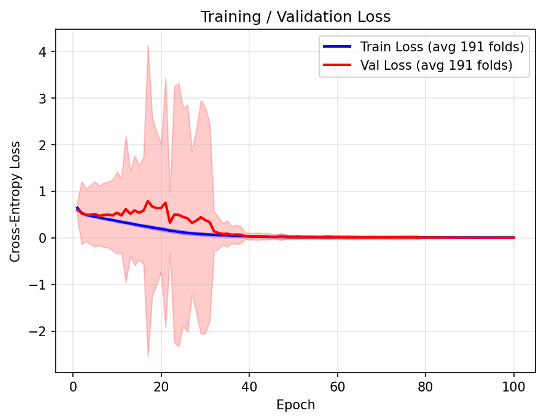
\includegraphics[width=\textwidth]{figures/2020_agcn_loss.png}
        \caption{2020 (LOOCV)}
        \label{fig:gcn_loss_2020}
    \end{subfigure}
    \hfill
    \begin{subfigure}[t]{0.32\textwidth}
        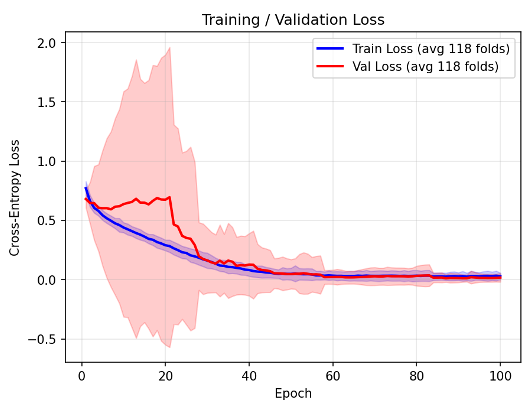
\includegraphics[width=\textwidth]{figures/2025_agcn_loss.png}
        \caption{2025 (LOOCV)}
        \label{fig:gcn_loss_2025}
    \end{subfigure}
    \hfill
    \begin{subfigure}[t]{0.32\textwidth}
        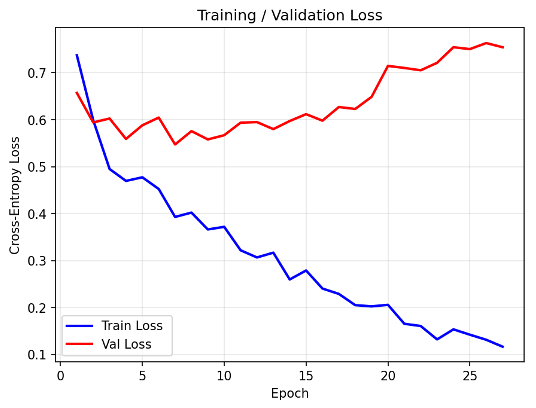
\includegraphics[width=\textwidth]{figures/cross_agcn_loss.png}
        \caption{Cross-cohort}
        \label{fig:gcn_loss_cross}
    \end{subfigure}
    \caption{Training and validation loss curves of AGCN.}
    \label{fig:gcn_loss_comparison}
\end{figure}

\begin{figure}[H]
    \centering
    \begin{subfigure}[t]{0.32\textwidth}
        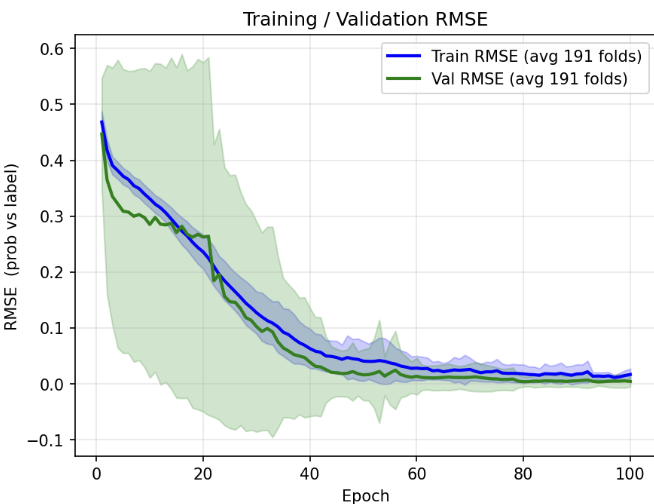
\includegraphics[width=\textwidth]{figures/2020_agcn_rmse.png}
        \caption{2020 (LOOCV)}
        \label{fig:gcn_rmse_2020}
    \end{subfigure}
    \hfill
    \begin{subfigure}[t]{0.32\textwidth}
        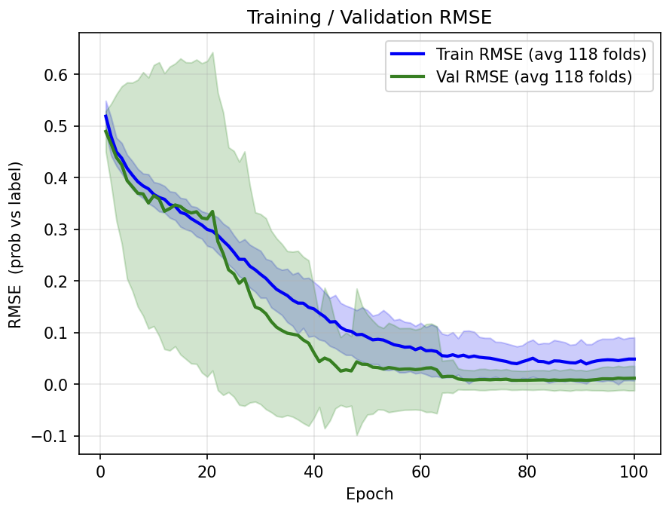
\includegraphics[width=\textwidth]{figures/2025_agcn_rmse.png}
        \caption{2025 (LOOCV)}
        \label{fig:gcn_rmse_2025}
    \end{subfigure}
    \hfill
    \begin{subfigure}[t]{0.32\textwidth}
        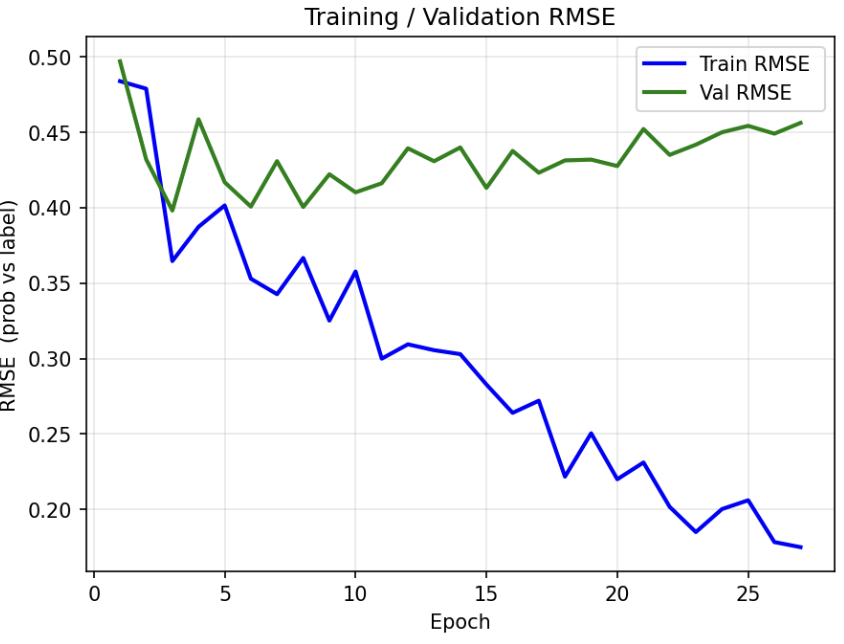
\includegraphics[width=\textwidth]{figures/cross_agcn_rmse.png}
        \caption{Cross-cohort}
        \label{fig:gcn_rmse_cross}
    \end{subfigure}
    \caption{Root Mean Square Error (RMSE) curves of AGCN across training epochs.}
    \label{fig:gcn_rmse_comparison}
\end{figure}

\subsection{Observation}

Within cohort, AGCN dominates every hand-crafted configuration from Experiments~2--4, reaching AUROCs of $0.98$ on both the 2020 and 2025 cohorts with accuracies of $0.92$--$0.93$ and F1-scores of $0.85$--$0.89$.

The loss and RMSE curves in Figs.~\ref{fig:gcn_loss_comparison} and~\ref{fig:gcn_rmse_comparison} provide important context for interpreting this result. Under LOOCV, each validation fold contains exactly one subject, so the per-fold validation loss is a single-sample measurement: when the model predicts that subject correctly the loss approaches zero, and when it fails the loss can be arbitrarily large. Averaged across all folds, both the mean training loss and the mean validation loss converge to near zero by epoch~100, and the validation RMSE likewise decays toward zero. This structural property of single-sample LOOCV means that the near-perfect within-cohort AUROC reflects the model's ability to classify each individual held-out subject after training on a near-complete cohort, rather than generalisation to a held-out distribution. The shaded variance bands further illustrate this: the 2020 cohort exhibits substantially wider per-fold variation (band spanning roughly $-2$ to $+4$ in the early epochs) than the 2025 cohort (band spanning roughly $0$ to $2$), consistent with the more heterogeneous video durations and recording conditions of the 2020 protocol relative to the standardised 30-second 2025 recordings.

In the cross-cohort transfer setting, the loss curves tell a qualitatively different story. The training loss decreases monotonically from $0.73$ to $0.12$, whereas the test-cohort loss rises steadily from approximately $0.60$ at epoch~1 to $0.75$ at the point of early stopping (epoch~$\approx 27$), yielding the classic diverging pattern of overfitting. The corresponding cross-cohort RMSE does not converge but oscillates and trends upward, ending near $0.46$, indicating that the model's probability estimates on the 2025 cohort become progressively less calibrated as training continues on the 2020 source distribution. Consequently, AGCN drops to an AUROC of $0.59$, an accuracy of $0.46$, and an F1-score of $0.40$, falling behind every hand-crafted configuration in Table~\ref{tab:gcn_cross_dataset}.

This sharp reversal from within-cohort to cross-cohort performance suggests that the adaptive graph topology learned from the 2020 training data may capture patterns that are specific to that cohort's distribution and do not generalise well to the 2025 recording protocol or patient population. One plausible contributing factor is that the graph adjacency is re-estimated from the node features of each training sample, so the discovered joint relationships may be sensitive to cohort-level differences in recording conditions, subject demographics, or movement characteristics; a sufficiently large distribution shift could invalidate the learned topology. Another likely factor is the small clinical dataset size, which provides limited headroom for the model to learn cohort-invariant representations: under LOOCV each fold trains on a near-complete cohort, favouring memorisation over generalisation. Taken together, these factors offer a plausible account of why AGCN underperforms the hand-crafted baselines in cross-cohort evaluation, although the relative contribution of each factor cannot be isolated from this experiment alone.
